\section{Fujitsu}
\label{sec_fujitsu}

% vortragFujitsu
% Karsten Beins, Vortrag am Hasso-Plattner-Institut im Rahmen des Industrie-Seminars zum Cloud-Computing, 2014
%
% - Fujitsu
%	- führendes japanisches Unternehmen für Informations- und Kommunikationstechnik
%	- viertgrößter IT-Dienstleister der Welt
%	- Philosophie: Mensch im Mittelpunkt (Human-Centric Paradigm)
%		- Creativität, Flexibilität, Innovation...

\IEEEPARstart{F}{ujitsu}\footnote{\url{http://www.fujitsu.com/}} ist das führende japanische Unternehmen für Informations- und Kommunikationstechnik und zudem der viertgrößte IT-Dienstleister der Welt. 

\subsection{Herausforderungen des Cloud Computing}
\label{sec_fujitsu_general}

% - Cloud
%	- hat sich von Hype zu Megatrend entwickelt 
%	-> Bild zu Gartner-Hype-Cycle 2014 (http://www.gartner.com/newsroom/id/2819918)
% - Probleme mit Cloud
%	- aus technischer Sicht kein Problem (Modelle etc. mittlerweise vorhanden)
%	- für Business-Kunden: schwieriger Weg zur geeigneten Lösung

Im Folgenden werden die im Vortrag von Karsten Beins\cite{vortragFujitsu} dargelegten Ansichten zum Cloud Computing zusammengefasst.

Cloud Computing hat sich vom Hype zum Megatrend entwickelt. 
Wie im Gartner-Hype-Cycle von 2014, zu sehen in Abbildung \ref{fig:gartnerHypeCycle2014}, ersichtlich ist, befindet sich Cloud Computing im Allgemeinen auf dem Weg von der Desillusionierung zur Reife. 

\begin{figure*}
	\centering
	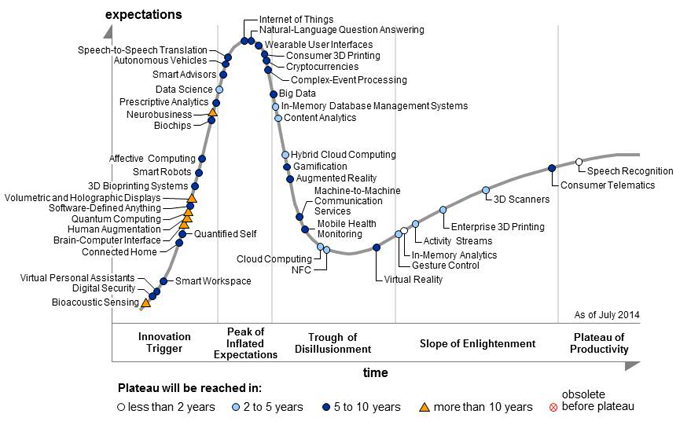
\includegraphics[width=0.8\linewidth]{images/gartnerHypeCycle2014}
	\caption{Gartner Hype Cycle 2014. http://www.gartner.com/newsroom/id/2819918, Zugriff 22.03.2015}
	\label{fig:gartnerHypeCycle2014}
\end{figure*}

In technischer Hinsicht existieren für die Umsetzung von Cloud-Anwendungen bereits etablierte Modelle und Möglichkeiten. 
Für Business-Kunden ist es jedoch weiterhin schwierig, den Weg zu einer geeigneten Cloud-Lösung zu finden. 
So gibt es verschiedene Herausforderungen für Unternehmen, welche Cloud Computing verwenden wollen.

% - identifizierte Herausforderungen für Unternehmen, die Cloud verwenden wollen
%	- Datensicherheit: manche Daten müssen unter eigener Kontrolle bleiben (z.B. gesetzliche Regelungen)
%	- Datenschutz: werden Sicherheitsvorkehrungen vom Cloud-Anbieter umgesetzt? Gesetze wie der amerikanische Patriot-Act
%	- Kontrolle: wirksame Abgrenzung verschiedener Cloud-Kunden bei geteilter Infrastruktur
%	- Flexibilität: Entwicklung neuer Lösungen könnte mehr Flexibilität / Schutz erfordern, als für gewöhnlich möglich ist
%	- Komplexität
%		- Mehrzahl bestehender Applikationen nicht für Cloud ausgelegt
%		- komplexe Anwendungstopologien -> Deployment, Skalierung, Lifecycle Management, Migration zu / zwischen Cloud, Verfügbarkeit, Robustheit schwierig
%		- Unternehmensapplikationen in die Cloud verschieben
%			- einfach und erprobt: einzelne Applikationen
%			- schwierig: eng miteinander vernetzte und komplexe Kernapplikationen
%	- Integration: Interaktion zwischen Anwendungen in verschiedenen Clouds und klassischer IT-Infrastruktur
%	- Kosten: Voraussage der Kosten, vorteilhafte Applikationen
%	- Kenntnisse: Wissen erwerben, um mit diesen Herausforderungen umzugehen

\begin{description}
  \item[Datensicherheit] \hfill \\
  Hiermit ist gemeint, dass formale Ansprüche an die Speicherung von Daten gestellt werden, wie sie zum Beispiel durch gesetzliche oder unternehmensinterne Regelungen gegeben sind, etwa in Form einer regionalen Begrenzung.
  \item[Datenschutz] \hfill \\
  Es muss sichergestellt werden, dass kein Unbefugter Zugriff auf die Daten des Anwenders hat. Besorgniserregend können hierbei gesetzliche Regelungen sein, die beispielsweise den Cloud-Anbieter zwingen, ausländischen Behörden Zugang zu gewähren.
  \item[Kontrolle] \hfill \\
  Die Infrastruktur eines Cloud-Anbieters kann gegebenenfalls von mehreren Kunden gleichzeitig genutzt werden. Hierbei dürfen sich die Kunden nicht auf unerwünschte Weise gegenseitig beeinträchtigen.
  \item[Flexibilität] \hfill \\
  Für gewisse Anwendungsfälle, wie beispielsweise der Entwicklung neuer Anwendungen, mag die vom Cloud-Anbieter bereitgestellte Lösung nicht flexibel genug sein.
  \item[Komplexität] \hfill \\
  Anwendungen eines Unternehmens kommen mitunter mit komplexen Topologien einher und sind nicht zwangsläufig auf die Ausführung in der Cloud ausgelegt. Einzelne Applikationen können auf erprobte Art und Weise in die Cloud migriert werden, was für komplexe und eng vernetzte Anwendungen deutlich schwieriger sein kann. Deployment, Skalierung, Lifecycle Management, Migration zu und zwischen Clouds, Verfügbarkeit und Robustheit müssen ermöglicht werden.
  \item[Integration] \hfill \\
  Es muss ermöglicht werden, dass Anwendungen in der Cloud oder in unterschiedlichen Clouds miteinander sowie mit Anwendungen außerhalb der Cloud interagieren können.
  \item[Kosten] \hfill \\
  Die Kosten, die mit der Verwendung einer Cloud-Lösung einhergehen, müssen voraussagbar sein. Zudem ist es möglich, dass manche Anwendungen im Hinblick auf die verursachten Kosten günstiger sind als andere.
  \item[Kenntnisse] \hfill \\
  Der Kunde muss das notwendige Wissen erlangen, um eine Cloud-Lösung angesichts der genannten Herausforderungen umsetzen zu können.
\end{description}

% - Schlussfolgerungen (laut Vortrag)
%	- Abwägungen für Anwender, z.B.
%		- Servicemodell:
%			- Vereinfachung durch Abstraktion: PaaS, SaaS
%			- Flexibilität, feingranulare Kontrolle: IaaS
%		- Betriebsmodell:
%			- Preis, Skalierbarkeit: public clouds
%			- Datensicherheit, -schutz: on-premise / hosted private cloud

An Schlussfolgerungen aus den oben genannten Herausforderungen wird genannt, dass Anwender bei der Wahl der passenden Cloud-Modelle abwägen müssen, worauf sie mehr Wert legen. 
So bieten im Hinblick auf die Service-Modelle Platform as a Service sowie Software as a Service eine einfachere Handhabung durch Abstraktion, während Infrastructure as a Service eine hohe Flexibilität und feingranulare Kontrolle ermöglicht. 
Hinsichtlich der Betriebsmodelle sind Public Clouds tendenziell günstiger und bieten eine bessere Skalierbarkeit, während On-Premise beziehungsweise Hosted Private Clouds geeigneter sind, hohe Anforderungen an Datensicherheit und -schutz umzusetzen.

\subsection{Service-Modelle}
\label{sec_fujitsu_delivery}

Fujitsu bietet Lösungen zu Infrastructure as a Service, Platform as a Service und Software as a Service. 
Die verschiedenen Varianten, um Infrastructure as a Service umzusetzen, werden in Abschnitt\ref{sec_fujitsu_deployment} erläutert.
...

\subsection{Betriebsmodelle}
\label{sec_fujitsu_deployment}

% Bild zu Modellen, http://www.fujitsu.com/global/services/infrastructure/iaas/

\begin{figure*}
	\centering
	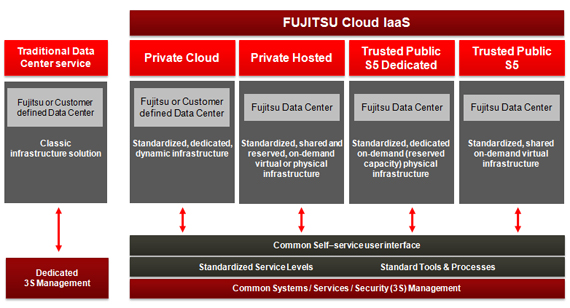
\includegraphics[width=0.8\linewidth]{images/fujitsuModels}
	\caption{Übersicht zu den Betriebsvarianten für Infrastructure as a Service von Fujitsu. \cite{fujitsuIaaS}}
	\label{fig:fujitsuModels}
\end{figure*}

Im Zusammenhang mit Infrastructure as a Service bietet Fujitsu verschiedene Betriebsmodelle\cite{fujitsuIaaS}, welche in Abbildung \ref{fig:fujitsuModels} dargestellt sind. Mit Trusted Public S5 bietet Fujitsu eine Public Cloud, welche skalierbare Ressourcen bei nutzungsabhängigen Kosten bietet und Vorteile hinsichtlich Zuverlässigkeit, Verfügbarkeit und Sicherheit bietet. Auch Trusted Public S5 Dedicated ist eine Public Cloud Lösung, die jedoch die exklusive Reservierung physischer Kapazitäten ermöglicht. 
